\documentclass[11pt]{article}
\usepackage{listings}
\lstset{
}

\usepackage{fancyhdr}
\pagestyle{fancy}
\newcommand\course{CSC 486B}
\newcommand\hwnumber{1}
\newcommand\duedate{January 14, 2020}

\lhead{Oliver Tonnesen\\V00885732}
\chead{\textbf{\Large Assignment \hwnumber}}
\rhead{\course\\\duedate}

\usepackage{graphicx}

\usepackage{mathtools}
\usepackage{amsmath}


\begin{document}
\stepcounter{section}
\section{Preliminaries: math} % Section 2
\subsection{Basic calculus} % Section 2.1
\subsubsection{} % Question 2.1.1
\[\frac{\partial y}{\partial x}=2ax+b\]


\subsubsection{} % Question 2.1.2
\[\frac{\partial y}{\partial x}=\cos^2x-\sin^2x\]


\subsubsection{} % Question 2.1.3
\[\frac{\partial y}{\partial x}=\frac{e^{-x}}{(1+e^{-x})^2}\]


\subsubsection{} % Question 2.1.4
\begin{align*}
	\frac{\partial y}{\partial x}
	&=\frac{e^x+e^{-x}}{e^x+e^{-x}}-\frac{(e^x-e^{-x})^2}{(e^x+e^{-x})^2}\\
	&=1-\left(\frac{e^x-e^{-x}}{e^x+e^{-x}}\right)^2\\
\end{align*}


\subsection{Taylor expansion} % Section 2.2
\subsubsection{} % Question 2.2.1
\[y=e^b+ae^bx+\frac{a^2e^bx^2}{2}+\frac{a^3e^{a\xi+b}x^3}{6},\xi\in[0,x]\]


\subsubsection{} % Question 2.2.2
\[y=\cos b+a\cos bx+\frac{a^2\cos b}{2}x^2+\frac{a^3\cos(a\xi+b)}{6}x^3,\xi\in[0,x]\]


\subsection{Matrix multiplication} % Section 2.3
\subsubsection{} % Question 2.3.1
\[
\begin{pmatrix}
	9 & 8 & 7\\
	6 & 5 & 4\\
	3 & 2 & 1\\
\end{pmatrix}
\begin{pmatrix}
	-1\\
	2\\
	-1
\end{pmatrix}=
\begin{pmatrix}
	0\\
	0\\
	0
\end{pmatrix}
\]


\subsubsection{} % Question 2.3.2
\[
\begin{pmatrix}
	-2\\
	1\\
	-2
\end{pmatrix}
\begin{pmatrix}
	1 & -2 & 1
\end{pmatrix}=
\begin{pmatrix}
	-2 & 4 & -2\\
	1 & -2 & 1\\
	-2 & 4 & -2
\end{pmatrix}
\]


\subsection{Applying chain rule on vectors and matrices} % Section 2.4
\begin{align*}
	\frac{\partial y}{\partial\mathbf x}
	&=\frac{\partial \lVert\mathbf A^T\mathbf x-\mathbf b\rVert_2^2}{\partial\mathbf x}\\
	&=\frac{\partial (\mathbf A^T\mathbf x-\mathbf b)\cdot(\mathbf A^T\mathbf x-\mathbf b)}{\partial\mathbf x}\\
	&=2(\mathbf A^T\mathbf x-\mathbf b)^T%\cdot A^T
\end{align*}

\section{Preliminaries: programming} % Section 3
\stepcounter{subsection}
\subsection{Reading, display, and save an image} % Section 3.2
\begin{figure}[h]
	\begin{minipage}{0.5 \textwidth}
		\centering
		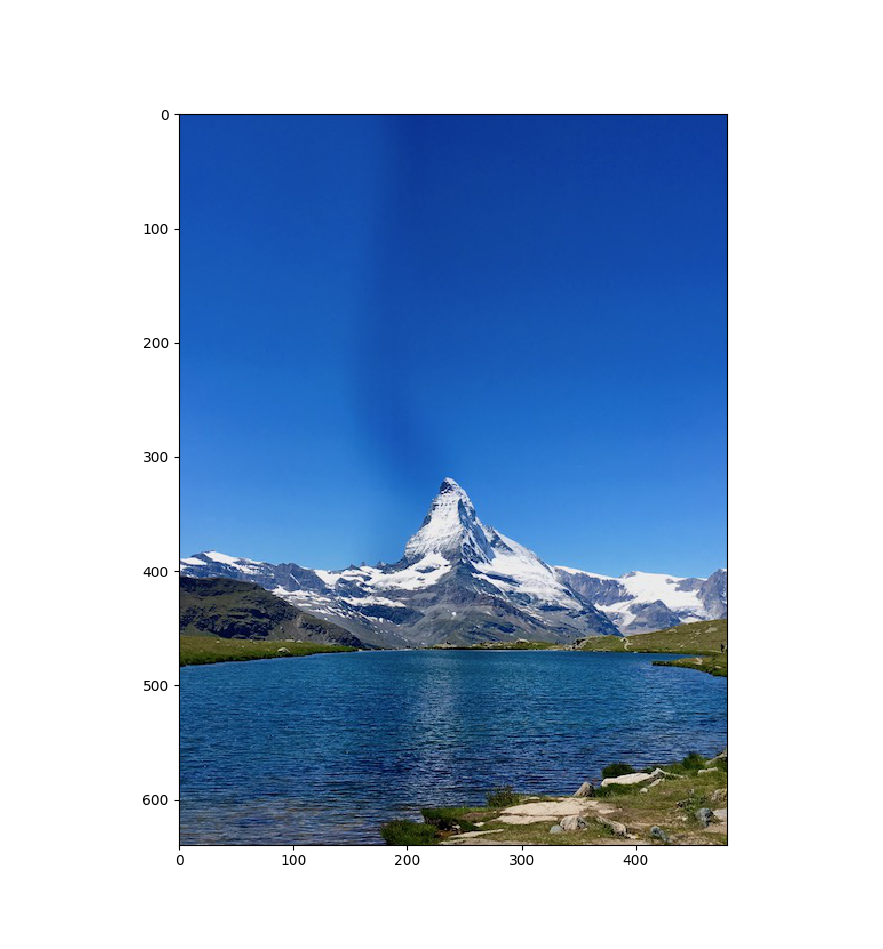
\includegraphics[width=1 \textwidth]{figures/original.png}
		\caption{Original image.}
	\end{minipage}
	\begin{minipage}{0.5 \textwidth}
		\centering
		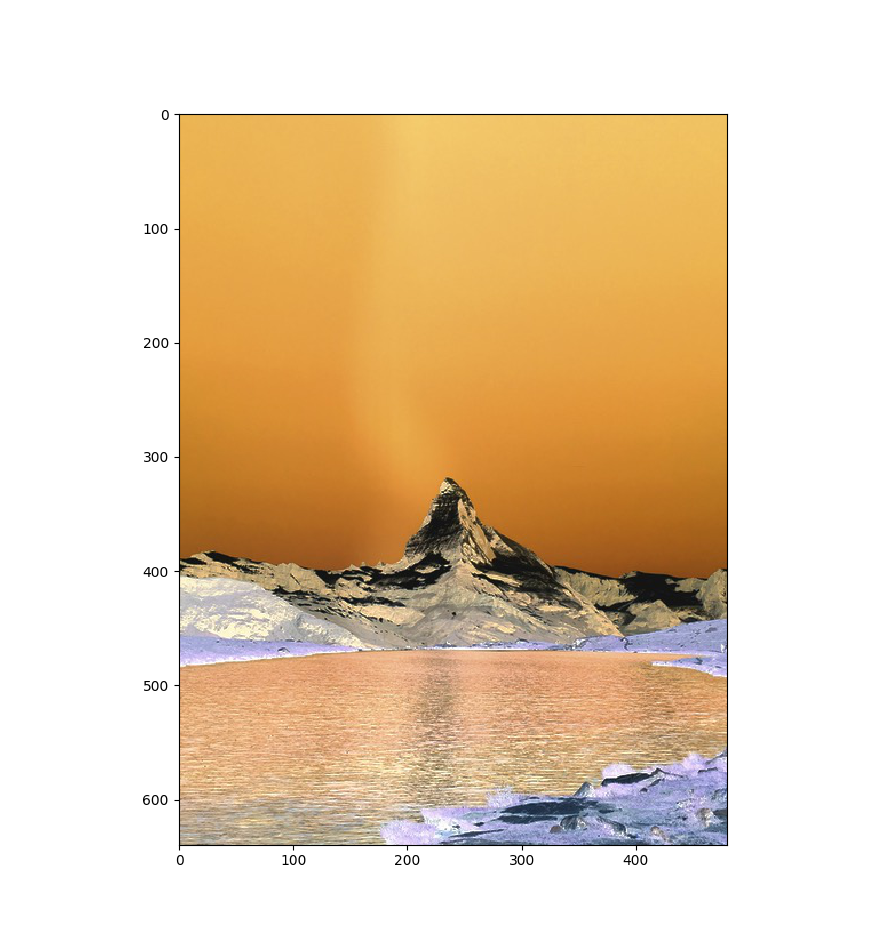
\includegraphics[width=1 \textwidth]{figures/inverted.png}
		\caption{Inverted image.}
\end{minipage}
\end{figure}
In this section I learned to open, manipulate, and display image files in Python.
The inverted image was obtained by subtracting the original image from a white image of the same size.


\subsection{Finding the edges of an image} % Section 3.3
This image was obtained by taking the difference of two Gaussian filtered copies of the original image.
\begin{figure}[h]
	\centering
	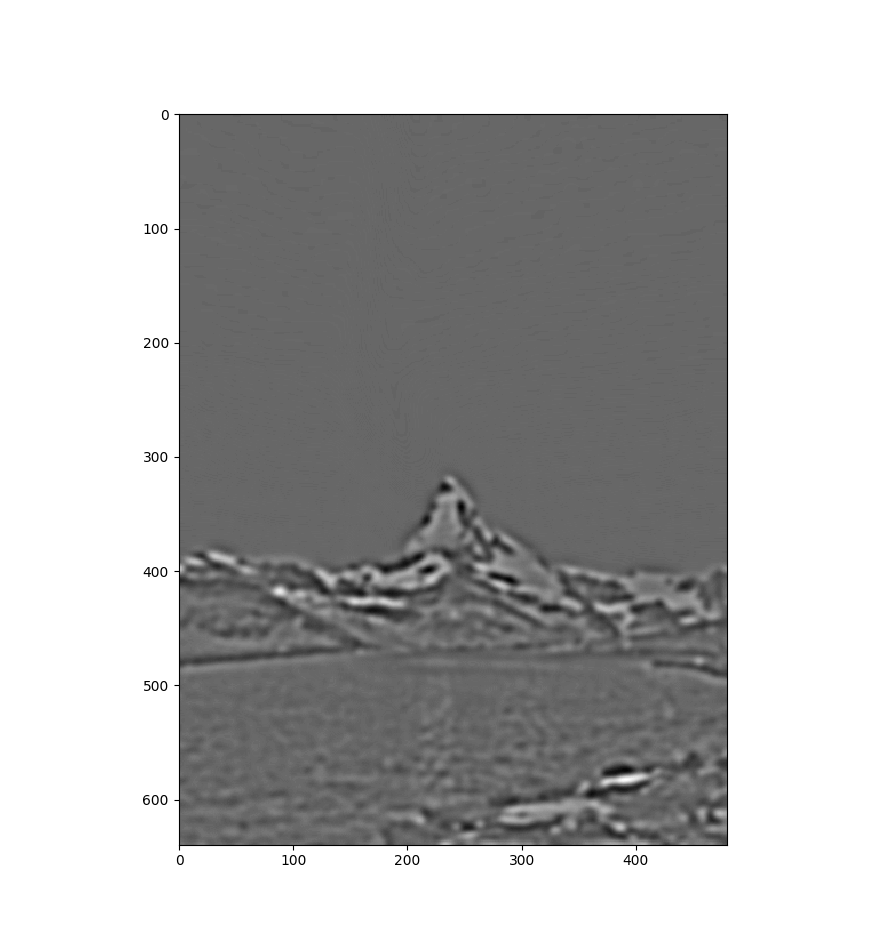
\includegraphics[width=0.6 \textwidth]{figures/edges.png}
	\caption{Difference of Gaussian filters.}
\end{figure}


\subsection{Thresholding} % Section 3.4
The image from the previous section was used to create the following image by turning the least intense 95\% of the pixels black.
\begin{figure}[h]
	\centering
	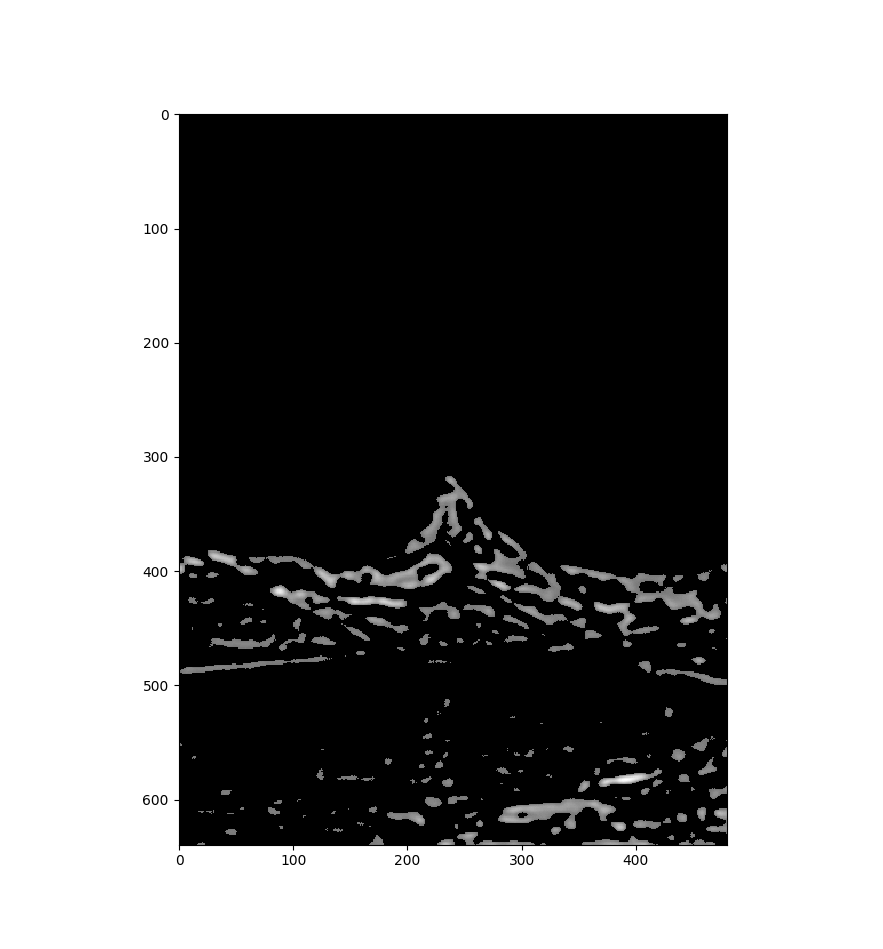
\includegraphics[width=0.6 \textwidth]{figures/thresholded.png}
	\caption{Thresholded image.}
\end{figure}


\end{document}
